\documentclass[conference]{IEEEtran}
\IEEEoverridecommandlockouts
% The preceding line is only needed to identify funding in the first footnote. If that is unneeded, please comment it out.
\usepackage{cite}
\usepackage{amsmath,amssymb,amsfonts}
\usepackage{algorithmic}
\usepackage{graphicx}
\usepackage{textcomp}
\usepackage{xcolor}
\usepackage[brazilian]{babel}
\usepackage[utf8]{inputenc}
\usepackage[T1]{fontenc}
\usepackage{listings}
\usepackage{color}
\usepackage{float}
\usepackage{multirow}

\definecolor{dkgreen}{rgb}{0,0.6,0}
\definecolor{gray}{rgb}{0.5,0.5,0.5}
\definecolor{mauve}{rgb}{0.58,0,0.82}

\lstset{frame=tb,
  language=Java,
  aboveskip=3mm,
  belowskip=3mm,
  showstringspaces=false,
  columns=flexible,
  basicstyle={\small\ttfamily},
  numbers=none,
  numberstyle=\tiny\color{gray},
  keywordstyle=\color{blue},
  commentstyle=\color{dkgreen},
  stringstyle=\color{mauve},
  breaklines=true,
  breakatwhitespace=true,
  tabsize=3
}
\lstset{language=Python}
\def\BibTeX{{\rm B\kern-.05em{\sc i\kern-.025em b}\kern-.08em
    T\kern-.1667em\lower.7ex\hbox{E}\kern-.125emX}}
\begin{document}

\title{Relatório do Laboratório 3: \\ Otimização com Métodos de Busca Local\\
}

\author{\IEEEauthorblockN{Isabelle Ferreira de Oliveira}
\IEEEauthorblockA{\textit{CT-213 - Engenharia da Computação 2020} \\
\textit{Instituto Tecnológico de Aeronáutica (ITA)}\\
São José dos Campos, Brasil \\
isabelle.ferreira3000@gmail.com}
}

\maketitle

\begin{abstract}
Esse relatório documenta a implementação dos seguintes algoritmos de otimização baseados em busca local: Descida do Gradiente, Hill Climbing e Simulated Annealing. Esses métodos foram testados em uma regressão linear para obter parâmetros físicos relativos ao movimento de uma bola. Por fim, os resultados das três implementações foram comparados.
\end{abstract}

\begin{IEEEkeywords}
Algoritmos de Otimização, busca local, Descida do Gradiente, Hill Climbing, Simulated Annealing, regressão linear
\end{IEEEkeywords}

\section{Introdução}
Otimização consiste em encontrar o mínimo (ou máximo) de uma função, ou seja, encontrar o conjunto de parâmetros que levem essa função ao seu mínimo (ou máximo). Também pode ser visto como encontrar a melhor solução dentre todas as soluções viáveis. Nesses problemas de otimização também é possível haver restrições acerca dos parâmetros que serão analisados.

Quando não se é possível encontrar essa solução de forma analítica, podem ser utilizados métodos numéricos. Dentre esses, estão algoritmos da classe de Metaheurísticas, que testam um número alto de soluções, conduzindo seus testes de forma a convergirem em alguma solução otimizada. 

Um exemplo famoso de solução analítica é o Método dos Mínimos Quadrados (MMQ). Já exemplos de algoritmos da classe de Metaheurísticas são o Descida do Gradiente, o Hill Climbing e o Simulated Annealing. 

Os pseudo-códigos desses algoritmos de Metaheurísticas podem ser vistos nas subseções a seguir. Em seguida, será apresentado como esses algoritmos foram implementados no contexto do laboratório.

\subsection{Descida do Gradiente}
\begin{lstlisting}
def gradient_descent(dJ, theta, alpha):
	while not check_stopping_condition():
		theta = theta - alpha * dJ(theta)
	return theta
\end{lstlisting}

\subsection{Hill Climbing}
\begin{lstlisting}
def hill_climbing(J, theta):
	while not check_stopping_condition():
		best = None # J(None) = inf
		for neighbor in neighbors(theta):
			if J(neighbor) < J(best):
				best = neighbor
		if J(best) > J(theta):
			return theta
		theta = best
	return theta
\end{lstlisting}

\subsection{Simulated Annealing}
\begin{lstlisting}
def simulated_annealing(J, theta):
	while not check_stopping_condition():
		T = temperature_schedule(i)
		if T < 0.0:
			return theta
		neighbor = random_neighbor(theta)
		deltaE = J(neighbor) - J(theta)
		if deltaE < 0:
			theta = neighbor
		else:
			r = random_uniform(0.0, 1.0) # Draws random number w/ uniform dist.
			if r <= exp(-deltaE / T):
			theta = neighbor
	return theta
\end{lstlisting}

\section{Implementação dos algoritmos}
Na parte relativa a implementação dos algoritmos de busca, era necessário preencher os códigos das funções \textit{dijkstra}, \textit{greedy} e \textit{a\underline{\space}star} da classe \textit{PathPlanner} do código base fornecido \cite{b1}.

A análise de vários pontos dos algoritmos descritos acima terão uma breve descrição em alto nível da sua implementação a seguir. 

Como os algoritmos foram implementados em Python, as filas de prioridade foram importadas da biblioteca \textit{heapq}, sendo utilizado as funções \textit{heappush} e \textit{heappop} para adicionar e retirar um elemento da fila, respectivamente.

Já as funções heurísticas dos algoritmos Greedy e A* foram calculadas a partir da função \textit{distance\underline{\space}to}, que calcula a distância euclidiana entre um nó específico e o nó objetivo. Essa função já foi fornecida pelo código básico.

Na etapa de percorrer os sucessores de um determinado nó para se calcular os custos relativos aquele caminho analisado, utilizou-se a função \textit{get\underline{\space}successors} para se obter esses sucessores. Para cada nó analisado, então, seu nó sucessor foi adicionado à fila de prioridade, sendo o custo dependente se o movimento se deu pela diagonal ou pela lateral do nó do \textit{grid}. Dessa forma, passos laterais tiveram custos menores que passos diagonais, na proporção de 1:$\sqrt{2}$. Uma representação de um nó específico do grafo e seus 8 vizinhos foi apresentado na Figura \ref{8-conectado}.

%\begin{figure}[htbp]
%\centerline{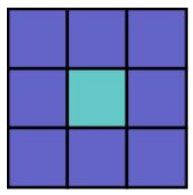
\includegraphics[scale=0.4]{8-conectado.png}}
%\caption{Representação de 8-conectado. Cada nó apresenta 8 vizinhos, sendo 4 laterais e 8 %diagonais.}
%\label{8-conectado}
%\end{figure}

Quando um determinado nó era, por fim, retirado da fila de prioridade, o custo mínimo do início do trajeto até aquele ponto já estaria definido. Nesse instante, então, o atributo \textit{closed} daquele nó foi setado como \textit{True}. Ao nó com custo definido de caminho do início até ele for o nó objetivo, a busca encerrou-se. No algoritmo Greedy, excepcionalmente, o custo já estava definido desde a primeira vez que o nó em específico era visitado.

\section{Resultados e Conclusões}
Os resultados das trajetórias de otimização obtidos após a execução das implementações dos algoritmos descritos acima foram apresentados nas Figuras \ref{gradient_descent}, \ref{hill_climbing} e \ref{simulated_annealing} para Descida do Gradiente, Hill Climbing e Simulated Annealing, respectivamente, e a sobreposição dessas trajetórias foi apresentada na Figura \ref{optimization_comparison} para melhor comparação visual.

\begin{figure}[htbp]
\centering
\centerline{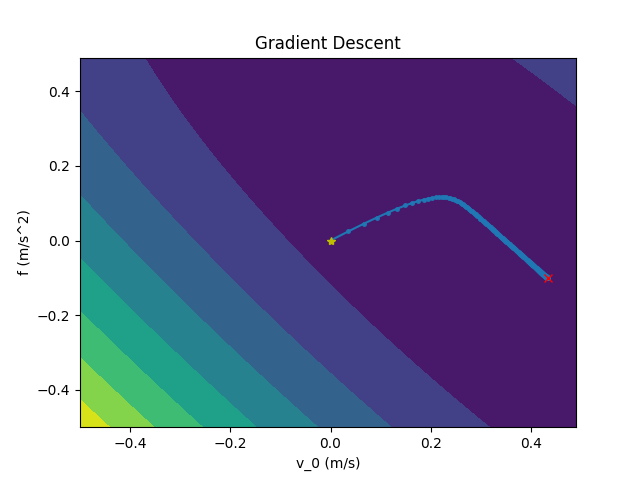
\includegraphics[scale=0.4]{gradient_descent.png}}
\caption{Trajetória de otimização usando Descida do Gradiente.}
\label{gradient_descent}
\end{figure}

\begin{figure}[htbp]
\centering
\centerline{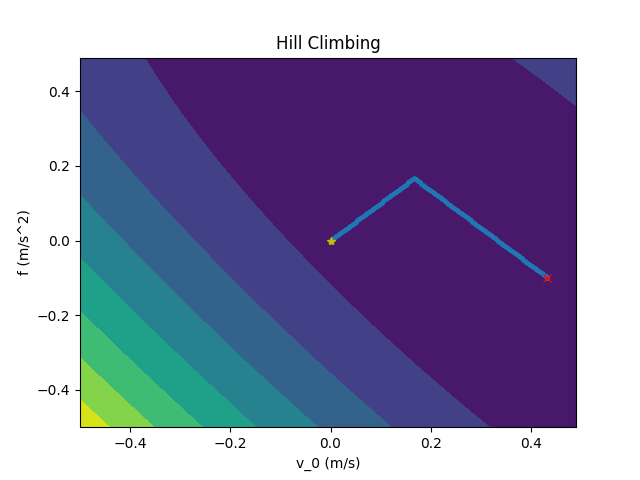
\includegraphics[scale=0.4]{hill_climbing.png}}
\caption{Trajetória de otimização usando Hill Climbing.}
\label{hill_climbing}
\end{figure} 

\begin{figure}[htbp]
\centering
\centerline{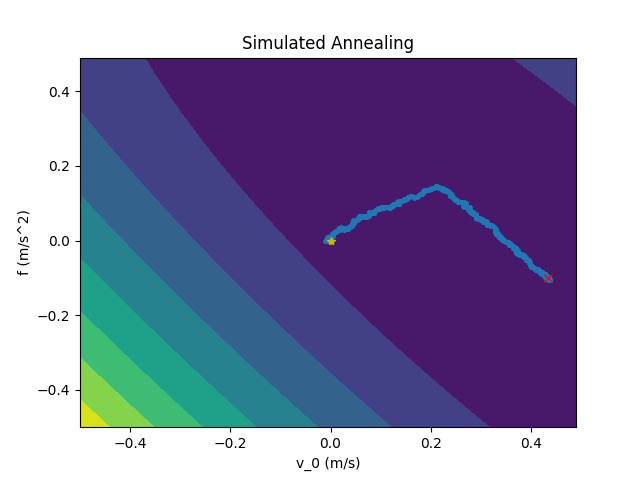
\includegraphics[scale=0.4]{simulated_annealing.png}}
\caption{Trajetória de otimização usando Simulated Annealing.}
\label{simulated_annealing}
\end{figure}

\begin{figure}[htbp]
\centering
\centerline{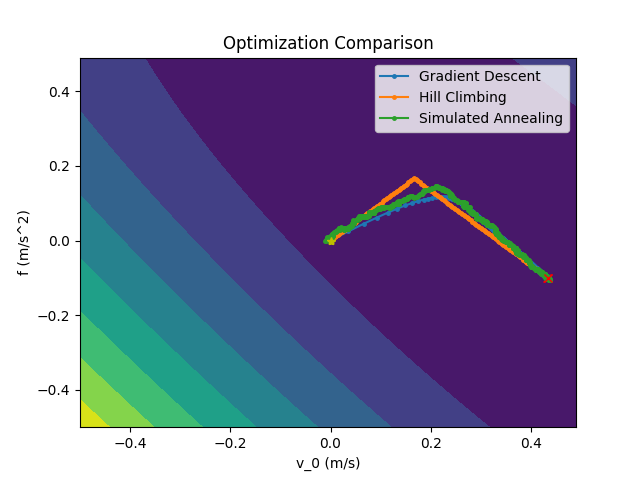
\includegraphics[scale=0.4]{optimization_comparison.png}}
\caption{Comparação de trajetórias de otimização usando Descida do Gradiente, Hill Climbing e Simulated Annealing.}
\label{optimization_comparison}
\end{figure}

Aplicando os valores encontrados para os parâmetros $v_0$ e $f$, o gráfico de velocidade da bola por tempo foi apresentado na Figura \ref{fit_comparison}. Esses valores numéricos de $v_0$ e $f$ podem ser vistos na Tabela \ref{tabelaX} para cada método estudado nesse laboratório, além do resultado fornecido inicialmente para o método de Mínimos Quadrados.

\begin{figure}[htbp]
\centering
\centerline{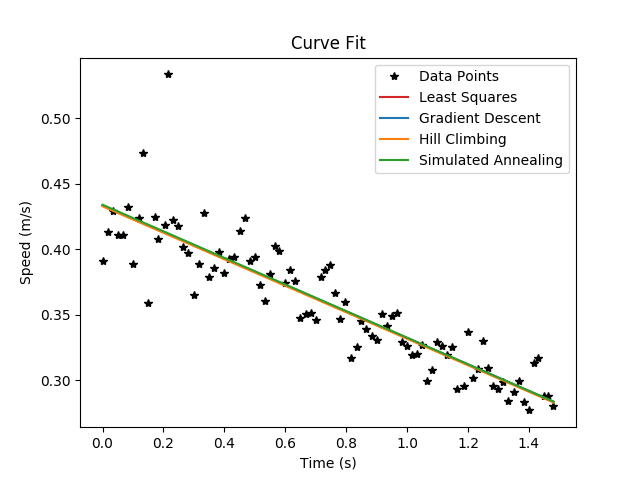
\includegraphics[scale=0.4]{fit_comparison.png}}
\caption{Comparação das regressões lineares das otimizações usando Descida do Gradiente, Hill Climbing e Simulated Annealing.}
\label{fit_comparison}
\end{figure}

Para os três casos, os algoritmos foram parados pelo critério de quantidade de iterações. Foram executadas, então, 1000 iterações para Descida do Gradiente e Hill Climbing, e 5000 para Simulated Annealing.

\begin{table}[htbp]
\centering
\caption{Comparação das soluções encontradas para os parâmetros físicos da bola para os algoritmos implementados no laboratório.}
\label{tabelaX}
\begin{tabular}{cc|c|c|c|c|l}
\cline{1-3}
\multicolumn{1}{ |c  }{\multirow{2}{*}{\textbf{Algoritmo}}} & 
\multicolumn{2}{ |c| }{\textbf{Solução}}
\\ \cline{2-3}
\multicolumn{1}{ |c  }{} & 
\multicolumn{1}{ |c  }{\textbf{$v_0$}} & 
\multicolumn{1}{ |c| }{\textbf{$f$}}
\\ \cline{1-3} 
\multicolumn{1}{ |c  }{Mínimos Quadrados} &
\multicolumn{1}{ |c  }{0.43337277} &
\multicolumn{1}{ |c| }{-0.10102096}
\\ \cline{1-3}
\multicolumn{1}{ |c  }{Descida do Gradiente} &
\multicolumn{1}{ |c  }{0.4333707} &
\multicolumn{1}{ |c| }{-0.10101849}
\\ \cline{1-3}
\multicolumn{1}{ |c  }{Hill Climbing} &
\multicolumn{1}{ |c  }{0.43274935} &
\multicolumn{1}{ |c| }{-0.10099495}
\\ \cline{1-3}
\multicolumn{1}{ |c  }{Simulated Annealing} &
\multicolumn{1}{ |c  }{0.43397656} &
\multicolumn{1}{ |c| }{-0.10134529}
\\ \cline{1-3}

\end{tabular}
\end{table}

Tendo em vista o que foi apresentado, pode-se notar, por fim, que esses algoritmos realmente se demonstraram eficazes em encontrar parâmetros otimizados para uma determinada função de custo e um ponto inicial de partida.

\begin{thebibliography}{00}
\bibitem{b1} M. Maximo, ``Roteiro: Laboratório 3 - Otimização com Métodos de Busca Local''. Instituto Tecnológico de Aeronáutica, Departamento de Computação. CT-213, 2019.
\end{thebibliography}

\end{document}
